\begin{figure}[h]
  \centering
  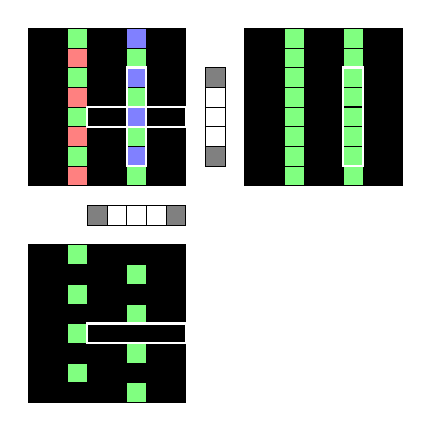
\begin{tikzpicture}
    \begin{scope}[shift={(-4,0)}, local bounding box = cfa]
      \begin{scope}[shift={(0,0)}]
        \filldraw[fill=green!50]   (0,0)     rectangle (1,1);
        \fill[fill=red!50]  (0,0)     rectangle (.25,.25);
        \fill[fill=red!50]  (.5,0)    rectangle (.75,.25);
        \fill[fill=red!50]  (.5,.5)   rectangle (.75,.75);
        \fill[fill=red!50]  (0,.5)    rectangle (.25,.75);
        \fill[fill=blue!50] (.25,.25) rectangle (.5,.5);
        \fill[fill=blue!50] (.75,.25) rectangle (1,.5);
        \fill[fill=blue!50] (.25,.75) rectangle (.5,1);
        \fill[fill=blue!50] (.75,.75) rectangle (1,1);
        \draw[step=.25,very thin] (0,0) grid (1,1);
      \end{scope}
      \begin{scope}[shift={(0,1)}]
        \filldraw[fill=green!50]   (0,0)     rectangle (1,1);
        \fill[fill=red!50]  (0,0)     rectangle (.25,.25);
        \fill[fill=red!50]  (.5,0)    rectangle (.75,.25);
        \fill[fill=red!50]  (.5,.5)   rectangle (.75,.75);
        \fill[fill=red!50]  (0,.5)    rectangle (.25,.75);
        \fill[fill=blue!50] (.25,.25) rectangle (.5,.5);
        \fill[fill=blue!50] (.75,.25) rectangle (1,.5);
        \fill[fill=blue!50] (.25,.75) rectangle (.5,1);
        \fill[fill=blue!50] (.75,.75) rectangle (1,1);
        \draw[step=.25,very thin] (0,0) grid (1,1);
      \end{scope}
      \begin{scope}[shift={(1,0)}]
        \filldraw[fill=green!50]   (0,0)     rectangle (1,1);
        \fill[fill=red!50]  (0,0)     rectangle (.25,.25);
        \fill[fill=red!50]  (.5,0)    rectangle (.75,.25);
        \fill[fill=red!50]  (.5,.5)   rectangle (.75,.75);
        \fill[fill=red!50]  (0,.5)    rectangle (.25,.75);
        \fill[fill=blue!50] (.25,.25) rectangle (.5,.5);
        \fill[fill=blue!50] (.75,.25) rectangle (1,.5);
        \fill[fill=blue!50] (.25,.75) rectangle (.5,1);
        \fill[fill=blue!50] (.75,.75) rectangle (1,1);
        \draw[step=.25,very thin] (0,0) grid (1,1);
      \end{scope}
      \begin{scope}[shift={(1,1)}]
        \filldraw[fill=green!50]   (0,0)     rectangle (1,1);
        \fill[fill=red!50]  (0,0)     rectangle (.25,.25);
        \fill[fill=red!50]  (.5,0)    rectangle (.75,.25);
        \fill[fill=red!50]  (.5,.5)   rectangle (.75,.75);
        \fill[fill=red!50]  (0,.5)    rectangle (.25,.75);
        \fill[fill=blue!50] (.25,.25) rectangle (.5,.5);
        \fill[fill=blue!50] (.75,.25) rectangle (1,.5);
        \fill[fill=blue!50] (.25,.75) rectangle (.5,1);
        \fill[fill=blue!50] (.75,.75) rectangle (1,1);
        \draw[step=.25,very thin] (0,0) grid (1,1);
      \end{scope}
      \fill[fill=black] (0,0) rectangle (.5,2);
      \fill[fill=black] (0.75,0) rectangle (1.25,2);
      \fill[fill=black] (1.5,0) rectangle (2,2);
      \draw[white, thick]  (1.25,.25) rectangle (1.5, 1.5);
      \draw[white, thick]  (.75,.75) rectangle (2, 1);
    \end{scope}
    \begin{scope}[shift={(-1.75, .25)}, local bounding box=exgreen1]
      \filldraw[fill=white]            (0,0)  rectangle (0.25,1.25);
      \fill[fill=black!50]         (0,0)  rectangle (.25,.25);
      \fill[fill=black!50]         (0,1)  rectangle (.25,1.25);
      \draw[black, step=.25,very thin] (0,0)  grid      (0.25,1.25);
      %\draw[black] (-0.25, 0) rectangle (.5, 1.25);
    \end{scope}
    \begin{scope}[shift={(-2, -0.5)}, rotate=90, local bounding box=exgreen1]
      \filldraw[fill=white]            (0,0)  rectangle (0.25,1.25);
      \fill[fill=black!50]         (0,0)  rectangle (.25,.25);
      \fill[fill=black!50]         (0,1)  rectangle (.25,1.25);
      \draw[black, step=.25,very thin] (0,0)  grid      (0.25,1.25);
    \end{scope}
    \begin{scope}[shift={(-1.25,0)}, local bounding box = cfaver]
      \begin{scope}[shift={(0,0)}]
        \filldraw[fill=green!50]   (0,0)     rectangle (1,1);
        \fill[fill=green!50]  (0,0)     rectangle (.25,.25);
        \fill[fill=green!50]  (.5,0)    rectangle (.75,.25);
        \fill[fill=green!50]  (.5,.5)   rectangle (.75,.75);
        \fill[fill=green!50]  (0,.5)    rectangle (.25,.75);
        \fill[fill=green!50] (.25,.25) rectangle (.5,.5);
        \fill[fill=green!50] (.75,.25) rectangle (1,.5);
        \fill[fill=green!50] (.25,.75) rectangle (.5,1);
        \fill[fill=green!50] (.75,.75) rectangle (1,1);
        \draw[step=.25,very thin] (0,0) grid (1,1);
      \end{scope}
      \begin{scope}[shift={(0,1)}]
        \filldraw[fill=green!50]   (0,0)     rectangle (1,1);
        \fill[fill=green!50]  (0,0)     rectangle (.25,.25);
        \fill[fill=green!50]  (.5,0)    rectangle (.75,.25);
        \fill[fill=green!50]  (.5,.5)   rectangle (.75,.75);
        \fill[fill=green!50]  (0,.5)    rectangle (.25,.75);
        \fill[fill=green!50] (.25,.25) rectangle (.5,.5);
        \fill[fill=green!50] (.75,.25) rectangle (1,.5);
        \fill[fill=green!50] (.25,.75) rectangle (.5,1);
        \fill[fill=green!50] (.75,.75) rectangle (1,1);
        \draw[step=.25,very thin] (0,0) grid (1,1);
      \end{scope}
      \begin{scope}[shift={(1,0)}]
        \filldraw[fill=green!50]   (0,0)     rectangle (1,1);
        \fill[fill=green!50]  (0,0)     rectangle (.25,.25);
        \fill[fill=green!50]  (.5,0)    rectangle (.75,.25);
        \fill[fill=green!50]  (.5,.5)   rectangle (.75,.75);
        \fill[fill=green!50]  (0,.5)    rectangle (.25,.75);
        \fill[fill=green!50] (.25,.25) rectangle (.5,.5);
        \fill[fill=green!50] (.75,.25) rectangle (1,.5);
        \fill[fill=green!50] (.25,.75) rectangle (.5,1);
        \fill[fill=green!50] (.75,.75) rectangle (1,1);
        \draw[step=.25,very thin] (0,0) grid (1,1);
      \end{scope}
      \begin{scope}[shift={(1,1)}]
        \filldraw[fill=green!50]   (0,0)     rectangle (1,1);
        \fill[fill=green!50]  (0,0)     rectangle (.25,.25);
        \fill[fill=green!50]  (.5,0)    rectangle (.75,.25);
        \fill[fill=green!50]  (.5,.5)   rectangle (.75,.75);
        \fill[fill=green!50]  (0,.5)    rectangle (.25,.75);
        \fill[fill=green!50] (.25,.25) rectangle (.5,.5);
        \fill[fill=green!50] (.75,.25) rectangle (1,.5);
        \fill[fill=green!50] (.25,.75) rectangle (.5,1);
        \fill[fill=green!50] (.75,.75) rectangle (1,1);
        \draw[step=.25,very thin] (0,0) grid (1,1);
      \end{scope}
      \fill[fill=black] (0,0) rectangle (.5,2);
      \fill[fill=black] (0.75,0) rectangle (1.25,2);
      \fill[fill=black] (1.5,0) rectangle (2,2);
      \draw[white, thick]  (1.25,.25) rectangle (1.5, 1.5);
    \end{scope}
    \begin{scope}[shift={(-4,-2.75)}, local bounding box = cfahor]
      \begin{scope}[shift={(0,0)}]
        \filldraw[fill=green!50]   (0,0)     rectangle (1,1);
        \fill[fill=black]  (0,0)     rectangle (.25,.25);
        \fill[fill=black]  (.5,0)    rectangle (.75,.25);
        \fill[fill=black]  (.5,.5)   rectangle (.75,.75);
        \fill[fill=black]  (0,.5)    rectangle (.25,.75);
        \fill[fill=black] (.25,.25) rectangle (.5,.5);
        \fill[fill=black] (.75,.25) rectangle (1,.5);
        \fill[fill=black] (.25,.75) rectangle (.5,1);
        \fill[fill=black] (.75,.75) rectangle (1,1);
        \draw[step=.25,very thin] (0,0) grid (1,1);
      \end{scope}
      \begin{scope}[shift={(0,1)}]
        \filldraw[fill=green!50]   (0,0)     rectangle (1,1);
        \fill[fill=black]  (0,0)     rectangle (.25,.25);
        \fill[fill=black]  (.5,0)    rectangle (.75,.25);
        \fill[fill=black]  (.5,.5)   rectangle (.75,.75);
        \fill[fill=black]  (0,.5)    rectangle (.25,.75);
        \fill[fill=black] (.25,.25) rectangle (.5,.5);
        \fill[fill=black] (.75,.25) rectangle (1,.5);
        \fill[fill=black] (.25,.75) rectangle (.5,1);
        \fill[fill=black] (.75,.75) rectangle (1,1);
        \draw[step=.25,very thin] (0,0) grid (1,1);
      \end{scope}
      \begin{scope}[shift={(1,0)}]
        \filldraw[fill=green!50]   (0,0)     rectangle (1,1);
        \fill[fill=black]  (0,0)     rectangle (.25,.25);
        \fill[fill=black]  (.5,0)    rectangle (.75,.25);
        \fill[fill=black]  (.5,.5)   rectangle (.75,.75);
        \fill[fill=black]  (0,.5)    rectangle (.25,.75);
        \fill[fill=black] (.25,.25) rectangle (.5,.5);
        \fill[fill=black] (.75,.25) rectangle (1,.5);
        \fill[fill=black] (.25,.75) rectangle (.5,1);
        \fill[fill=black] (.75,.75) rectangle (1,1);
        \draw[step=.25,very thin] (0,0) grid (1,1);
      \end{scope}
      \begin{scope}[shift={(1,1)}]
        \filldraw[fill=green!50]   (0,0)     rectangle (1,1);
        \fill[fill=black]  (0,0)     rectangle (.25,.25);
        \fill[fill=black]  (.5,0)    rectangle (.75,.25);
        \fill[fill=black]  (.5,.5)   rectangle (.75,.75);
        \fill[fill=black]  (0,.5)    rectangle (.25,.75);
        \fill[fill=black] (.25,.25) rectangle (.5,.5);
        \fill[fill=black] (.75,.25) rectangle (1,.5);
        \fill[fill=black] (.25,.75) rectangle (.5,1);
        \fill[fill=black] (.75,.75) rectangle (1,1);
        \draw[step=.25,very thin] (0,0) grid (1,1);
      \end{scope}
      \fill[fill=black] (0,0) rectangle (.5,2);
      \fill[fill=black] (0.75,0) rectangle (1.25,2);
      \fill[fill=black] (1.5,0) rectangle (2,2);
      \draw[white, thick]  (.75,.75) rectangle (2, 1);
    \end{scope}

  \end{tikzpicture}
  \caption{Illustration of the convolution used to interpolate green samples in AHD}
  \label{fig:green-dual-int}
\end{figure}

